\section{Phonemes}
In this project the focus is to understand basic transcription of beatboxing, meaning that only kick, snare and cymbal is researched throughout this study. In order to articulate the percussive vocal sounds in terminologies this study revealed mainly two important ways to do so, the IPA \citep{ipa,} and the Standard Beatboxing Notation, which are also briefly described in this chapter \citep{humanbeatboxing,}.


Sounds can be described as “phonemes”. However is a phoneme recognizer not particularly needed to be developed for this project as it is based on basic transcription of standard vocal emulations \citep{Janer_syllablingon}. That being mentioned, it is still important to remember that beatboxing can be a complex artform and if one should aim to transcribe complex beatboxing as vocal input, one would need a comprehensive systematic approach which could be somewhat facilitated by understanding and utilizing aspects of the IPA(International Phonetic Alphabet) \citep{ipa}, the Standard Beatboxing Notation, or a combination of both.


However can it be said that the most relevant articulation of phonemes for this project can be found in the Standard Beatboxing Notation (SBN), which were developed by Gavin Tyte and Mark Splinter, humanbeatbox.com in 2006, and was actually based on a “simplified” approach to the IPA. The technical characteristics of the phonemes used for notations (phonetic approach) is the way to describe the sounds used beatboxing, which basically have much in common with the IPA.


The four types of sound in beatboxing \citep{BeatboxBible}:

  \begin{itemize} 
	\item Plosives

	
	\textit{Plosives are sounds where one stop the airway and release sound. Often used for kicks and snares.}
  
	\item Fricatives
	
	
	\textit{Fricatives are continious sounds like “schhh”, “tsss”. Often used to imitate cymbals.}
	
	\item Clicks
	
	
	\textit{Clicks are more subtle sounds that are often used to imitate claps and snaps, but also subtle snares.}
	
	\item Oscillations
	
	\textit{Oscillations sounds are continious sounds imitating synthesized instruments and robotic sounds like vibratos and alarms.}
\end{itemize}

Each of these four groups of sounds can be described into further detailed characteristics and potential utilizabilily in transcription of beatboxing, but the main purpose of this chapter is mainly to get acquainted with the techniques and terminologies of beatboxing and an idea of the phonetic complexity. This information could be useful when taking further steps towards the development of a complex transcription of beatboxing, and to gain simple understanding of the auditory features of beatboxing.
\begin{figure}[h]
	\begin{center}
		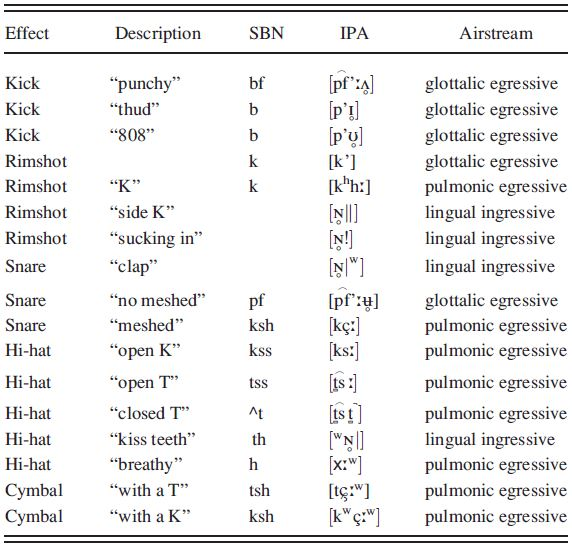
\includegraphics[height=5cm]{fig/phonemes.JPG}
		\caption{Illustration of phonemes utilized in Michael Proctors study on beatboxing \citep{proctor2012}}
		\label{VoiceBand}
	\end{center}
\end{figure}
